\documentclass[a4paper,12pt,english]{article}

\usepackage{babel}
\usepackage{graphicx}
\usepackage{listings}
\usepackage{color}
\usepackage{textcomp}
\definecolor{listinggray}{gray}{0.9}
\definecolor{lbcolor}{rgb}{0.95,0.95,0.95}
\lstset{
    backgroundcolor=\color{lbcolor},
    tabsize=4,
    rulecolor=,
    language=matlab,
        basicstyle=\scriptsize,
        upquote=true,
        aboveskip={1.5\baselineskip},
        columns=fixed,
        showstringspaces=false,
        extendedchars=true,
        breaklines=true,
        prebreak = \raisebox{0ex}[0ex][0ex]{\ensuremath{\hookleftarrow}},
        frame=single,
        showtabs=false,
        showspaces=false,
        showstringspaces=false,
        identifierstyle=\ttfamily,
        keywordstyle=\color[rgb]{0.1,0.1,0.6}\bfseries,
        commentstyle=\color[rgb]{0.133,0.545,0.133},
        stringstyle=\color[rgb]{0.627,0.126,0.941},
}

\newcommand{\fud}{\textbf{FuD}}
\newcommand{\cpp}{\texttt{C++}}
\renewcommand{\DJ}{\texttt{DistributableJob}}
\newcommand{\DJI}{\texttt{DistributableJobImplementation}}
\newcommand{\JU}{\texttt{JobUnit}}
\newcommand{\CP}{\texttt{ClientProcessor}}

\title{Using \fud \ to Develop a Distributed Application\\ \small{A Tutorial}}
\author{Guillermo J.~Biset}

\begin{document}

\maketitle

\section{About this document}

This document provides a simple tutorial to develop an application for the \fud \ framework. For a good description about \fud  \ and some interesting applications that use it you should see the thesis document instead of this one.

\section{Required knowledge}
To program a distributed application using \fud \ you don't need to know the intricacies of distributed programming, multithreading or any advanced topic in computer programming or computer science. However, some knowledge is necessary:
\begin{itemize}
 \item \cpp \ programming.
 \item Some basic Object Oriented programming concepts.
\end{itemize}

About \cpp \ programming, the definitive book on the subject comes from its creator: Bjarne Stroustrup\cite{cplusplus}. For good theory on Object Orientation and related topics, Bertrand Meyer has an excellent book on the subject\cite{oosc}.

\section{Basic \fud \ Topology}

There are two kinds of entities in a \fud \ application: the \textbf{Server} and the \textbf{Clients}. As their plurality suggests, for a particular running \fud \ application there will be exactly one server and many (or none) connected clients.

The \textbf{server} will be in charge of the overall status of the application and the \textbf{clients} will perform the basic computations needed to complete the work.

\section{Required \fud \ Concepts}

The purpose of \fud \ is to help a developer (be it an experienced one or not) solve a particular computational problem. So, if you are looking to use \fud, its because you have a problem to solve, and it can be solved by programming an application.

In turn, \fud \ is ideal if the problem is relatively simple, but a large amount of data must be manipulated.

Now, every application must perform work (or a Job) on some data (in this case, even doing nothing on no data could be considered as doing something).

In order to carry out work, some central notions from \fud \ must be comprehended:
\begin{description}
\item[Distributable Job]: A \DJ \ is an abstract work concept encapsulating any work that is to be performed. The notion is supposed to be taken as a \emph{large scale} job. Now, a property of these large scale jobs is that they can be subdivided into smaller jobs (or Job Units).
\item[Job Unit]: A \JU \ is an abstract work concept encapsulating a simple task to be performed. A \JU \ is atomic, therefore it cannot be subdivided into other Job Units. The task itself must be represented by a message, which will later be passed on to a processing client.
\item[Processing Client]: A \CP \ is a processing node. Its only task is to wait for messages, process them and, once finished, inform that the results are ready.
\end{description}

\subsection{The relationship of the Job Concepts}

The division of a \DJ \ is a \emph{transactional} process, meaning that if a \DJ \ produces a \JU \ then it must change state in some way, i.e. it must not produce the same \JU \ again.

In turn, \fud \ assures you that your \JU \ won't be forgotten. Under fair conditions of processing client availability and if the code to compute it terminates, every \JU \ will eventually be computed.

A \DJ \ can be decomposed into zero\footnote{Although a \DJ \ consisting of zero Job Units is not a useful thing.} or more\footnote{It is possible to have non terminating Distributable Jobs with an infinite amount of Job Units, which can be useful.} Job Units, and each \JU \ \emph{belongs to} a particular \DJ.

\subsection{Job States}

A \DJ \ may be in many different states, usually depending on the status of the data. The states and their meaning are:
\begin{description}
\item[ReadyToProduce]: The Job is ready to produce another Job Unit.
\item[WaitingMoreData]: The Job is waiting for more data or some event, can't produce a Job Unit at the moment.
\item[FinishedGenerating]: From here on, the Job won't produce any more Job Units.
\end{description}

It is your responsibility to know which of these states a \DJ \ is in. There is, nonetheless, a fourth (and very important) state for a \DJ: \emph{finished}. However, a \emph{finished} state is calculated automatically (i.e. you can't change when a \DJ \ is \emph{finished} or not) and is computed by the fact that the \DJ \ has \emph{FinishedGenerating} and all generated Job Units are \emph{Completed}. 

For Job Units, however, you don't need to know their state, but for reference, these are the possible ones:
\begin{description}
\item[Created]: The \JU \ hasn't been asigned to any \CP.
\item[Assigned]: The \JU \ has been asigned to one or more processing clients but none of them has, as of yet, returned the results of the computation.
\item[Completed]: At least one \CP \ has returned the results of the computation of this \JU.
\end{description}


\subsection{Job Responsibilities}

A \DJ \ must:
\begin{itemize}
 \item Know how to divide itself into a \JU.
 \item Know how to handle the results of a \JU.
 \item Know the state it is in.
\end{itemize}

Again, the division from a \DJ \ to a \JU \ must be \emph{transactional}, \fud \ will only call upon you to generate another \JU \ if you are in a \emph{ReadyToProduce} state. However, if by mistake or some obscure reason you can't produce a \JU \ when requested, there is a way for the corresponding method to return a non-\JU \ value\footnote{Since the method should return a pointer, a \texttt{NULL} value would suffice.}. 

The framework will call upon you to  handle the results of every \JU \ you generated only \textbf{once}, s  o you needn't worry about this when handling them.

As for the state, you should know that returning \emph{FinishedGenerating} once will unlink that \DJ \ from the processing part of the framework, but this does not mean that the \DJ \ itself has been completely computed (or \emph{finished}). 

On the other hand, a \JU \ must:
\begin{itemize}
\item Provide a message (a standard \texttt{string}) for a \CP.
\item Be able to inform its \textbf{size}, which is a user-defined (i.e. \textbf{you} define what it means) concept.
\end{itemize}

\section{Example: a simple counting application}

The problem we want to solve is as follows:

\begin{quote}
Develop a counting program that can count (one at a time) up to $N$. To do this, use $X$ Distributable Jobs, each of which will only count if it is its turn. Whose turn it is is identified simply: the $X$ jobs will be numbered from $0$ to $X-1$. Now, its the turn of job $x$ to count if and only if $n$(the current number up to which it has been counted) modulus $X$ equals $x$, or $n \% X = x$.
\end{quote}

An example could be the following. We want to count to $10$ with $7$ jobs ($\{0,1,2,3,4,5,6\}$). Initially, it will be the turn of job $0$ to count, so it will produce a \JU \ with the current number $n$ (which, obviouslly, is initially zero). Each \CP \ will deal with messages the same way, take the number and return it plus one. So, after a \JU \ is completed, the resulting number is stored as the current one. Now, after that first \JU \ is computed, $n$ will be $1$ and it is now the turn of job $1$ to go. When $n$ reaches $7$, it is the turn of job $0$ to go at it. This will go on until $N$ is reached.

\subsection{Implementing}

Ok, so, every application developer wishing to use \fud \ must implement the following:
\begin{itemize}
\item Every \DJ \ it needs, and all that entails.
\item The main application program (i.e. code containing the function \texttt{main}). Here you should include the header files for all the \DJ \ instances you defined and use the available methods for synchronizing.
\item A \CP \ to handle messages from \DJ \ instances.
\end{itemize}

Lets start then by implementing the only type of \DJ \ we have. Figure \ref{djdiag} shows the classes used to represent a \DJ. 

\begin{figure}[!ht]\label{djdiag}
\begin{center}
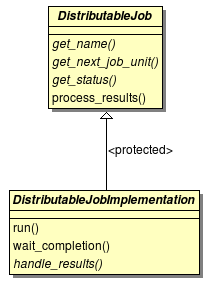
\includegraphics [bb= 0 0 211 286]{../design/graphics/Distributable-Jobs.png}
\end{center}
\caption{Class Diagram of the two classes used to represent Distributable Jobs.}
\end{figure}

You'll need to inherit from \DJI \ and reimplement the pure virtual methods declared in \DJ. The two methdos from \DJI \ are what you'll have at your disposal when implementing the \texttt{main} program.

The code from \DJ \ and the profile of the methods you need to implement are portrayed in table \ref{djcode}.

\begin{table}[!htb]
\lstset{language=C++}
\begin{lstlisting}[frame=single]
struct DistributableJob
{
  virtual void process_results(JobUnitID id, 
            const std::string* message) = 0;

  virtual JobUnit* get_next_job_unit(
                      JobUnitSize size) = 0;

  virtual DistributableJobStatus get_status() const= 0;
  
  virtual const char* get_name() const = 0;
};
\end{lstlisting}
\centering \caption{Class \DJ.} \label{djcode}
\end{table}

Table \ref{jucode} shows the code of a \JU \ abstraction. It should be declared private to the class that inherits from \DJI.

\begin{table}[!htb]
\lstset{language=C++}
\begin{lstlisting}[frame=single]
class JobUnit
{
  public:
    inline JobUnitID   get_id()   const {return _id;}
    inline JobUnitSize get_size() const {return _size;}

    virtual ~JobUnit(){};
  protected:
    JobUnit();

    void  set_size(JobUnitSize size);
  private:
    virtual const std::string&  get_message() const = 0;

    static JobUnitID _last_generated;
    JobUnitID        _id;
    JobUnitSize      _size;
};
\end{lstlisting}
\centering \caption{Class \JU.} \label{jucode}
\end{table}

Lets first implement our data, its only a database to hold a single number, the counting goal. Table \ref{dbheader} shows the header file for such a class.

\begin{table}[!htb]
\lstset{language=C++}
\begin{lstlisting}[frame=single]
#ifndef NUMBER_DATABASE_H
#define NUMBER_DATABASE_H

#include <cstdlib>

class NumberDatabase
{
    public:
        NumberDatabase(size_t up_to);

        size_t current_number() const;

        void update(size_t new_number);

        bool finished_counting() const;
    private:
        size_t _goal;
        size_t _n;
};

#endif
\end{lstlisting}
\centering \caption{Header file for \texttt{NumberDatabase} class.} \label{dbheader}
\end{table}

Its implementation is just as simple, table \ref{dbimpl} shows the source code. Note that the database doesn't know how to increment a number, it only supports a setter/getter pair for numbers, and remembers the counting goal to see when it has finished counting.

\begin{table}[!htb]
\lstset{language=C++}
\begin{lstlisting}[frame=single]
#include "number_database.h"

NumberDatabase::NumberDatabase(size_t up_to) :
    _goal(up_to),
    _n(0)
{
}

size_t NumberDatabase::current_number() const
{
    return _n;
}

void NumberDatabase::update(size_t new_number)
{
    _n = new_number;
}

bool NumberDatabase::finished_counting() const
{
    return _n >= _goal;
}
\end{lstlisting}
\centering \caption{Implementation file for \texttt{NumberDatabase} class.} \label{dbimpl}
\end{table}

Its now time to implement the actual \DJ, job \texttt{Counter}. In table \ref{counterhdr} you have the header file for it. Source code can be found in table \ref{countersrc}.

\begin{table}[!htb]
\lstset{language=C++}
\begin{tiny}
\begin{lstlisting}[frame=single]
#ifndef COUNTER_H
#define COUNTER_H

#include <string>

#include "fud.h"

#include "number_database.h"

using namespace fud;
class Counter : public DistributableJobImplementation
{
    public:
        Counter(NumberDatabase& num_db, size_t my_id);

        virtual ~Counter(){};
    private:
        virtual void        handle_results (JobUnitID id,InputMessage& input);

        virtual DistributableJobStatus get_status()    const;
        virtual const char*            get_name()      const;

        virtual JobUnit*    produce_next_job_unit(JobUnitSize size);

        static size_t   _job_count;

        size_t          _id;
        NumberDatabase& _num_db;

        size_t          _last;
};

#endif
\end{lstlisting}
\end{tiny}
\centering \caption{Header file for Counter \DJ.} \label{counterhdr}
\end{table}

\begin{table}[!htb]
\lstset{language=C++}
\begin{lstlisting}[frame=single]
#include <sstream>
#include "counter.h"

size_t Counter::_job_count = 0;

Counter::Counter(NumberDatabase& num_db, size_t my_id) :
    DistributableJobImplementation(),
    _id(my_id),
    _num_db(num_db),
    _last(my_id+1)
{
    ++_job_count;
}

const char* Counter::get_name() const
{
    std::ostringstream oss;
    oss << "Counter " << _id;
    return oss.str().c_str();
}

void Counter::handle_results (JobUnitID id,InputMessage& input)
{
    size_t count;
    input >> count;
    _num_db.update(count);
}

DistributableJobStatus Counter::get_status() const
{
    if (_num_db.finished_counting())
        return FinishedGenerating;
    else
        if ((_num_db.current_number() % _job_count == _id) &&
                     (_last != _num_db.current_number()) )
            return ReadyToProduce;
        else
            return WaitingMoreData;
}

JobUnit* Counter::produce_next_job_unit(JobUnitSize size)
{
    if ( get_status() == ReadyToProduce)
    {
        StreamingJobUnit* res = new StreamingJobUnit();

        (*res) << _num_db.current_number();
        res->set_size(1);

        _last = _num_db.current_number();

        return res;
    }
    else
        return NULL;
}
\end{lstlisting}
\centering \caption{Implementation file for the Counter \DJ.} \label{countersrc}
\end{table}

Finally, the source code that puts it all together via the main program can be found in table \ref{countermain}.

\begin{table}[!htb]
\lstset{language=C++}
\begin{lstlisting}[frame=single]
#include "counter.h"
#include "getopt_pp.h"

using namespace fud;
using namespace GetOpt;

int main(int argc, char** argv)
{
    size_t number(1000); //Default value.
    size_t jobs_n(5);    //Idem.

    GetOpt_pp ops(argc, argv);
    ops >> Option('n', "number", number) 
        >> Option('j',"jobs",jobs_n);

    NumberDatabase* db = new NumberDatabase(number);

    Counter* jobs[jobs_n];

    for (size_t i(0); i < jobs_n; ++i)
        jobs[i] = new Counter(*db,i);

    for (size_t i(0); i < jobs_n; ++i)
        jobs[i]->run();

    jobs[jobs_n-1]->wait_completion();

    std::cout << "Last number is: " //should be number
              << db->current_number() << std::endl;
}
\end{lstlisting}
\centering \caption{Main program of the \texttt{Counter} application.} \label{countermain}
\end{table}

Note that the implementation is very straightforward:
\begin{enumerate}
 \item Get the options passed by the user from the command line.
 \item Create the \DJ \ instances according to these options.
 \item Run each \DJ.
 \item Wait for the completion of each of them.
 \item Output results.
\end{enumerate}

Synchronization is achieved by the use of the methods \texttt{run()} (to start a distributable job) and \texttt{wait\_completion()} (to wait for its completion). In this case, all jobs run simultaneously (but they were started one at a time in order) and their completion is requested serially. We could, in this case, only request the completion of a single job, but it is better practice to ensure that all jobs are completed, thus avoiding inconsistencies between the data.

Last but not least, table \ref{counterclient} shows the main program of the client application and tables \ref{counterprochdr} and \ref{counterprocessor} the code of the actual \CP.

\begin{table}[!htb]
\lstset{language=C++}
\begin{lstlisting}[frame=single]
#include "distribution_client.h"
#include "counter_processor.h"
#include "getopt_pp.h"

using namespace fud;
using namespace GetOpt;

/* main program*/
int main(int argc, char** argv)
{
    size_t      port(31337);
    std::string address("127.0.0.1");

    GetOpt_pp ops(argc, argv);
    ops >> Option('a', "address", address) 
        >> Option('p', "port", port);

    new CounterProcessor();

    DistributionClient* distribution_client 
           = create_distribution_client(address,port);

    distribution_client->run();

    return 0;
}
\end{lstlisting}
\centering \caption{Main program of the \texttt{Counter} client application.} \label{counterclient}
\end{table}

\begin{table}[!htb]
\lstset{language=C++}
\begin{lstlisting}[frame=single]
#ifndef COUNTER_PROCESSOR_H
#define COUNTER_PROCESSOR_H

#include "fud.h"
#include "client_processor.h"
#include "job_unit.h"

namespace fud
{
    class CounterProcessor : ClientProcessor
    {
      public:
        CounterProcessor();

        virtual bool process(InputMessage& input, 
                             OutputMessage& output);
    };
}

#endif
\end{lstlisting}
\centering \caption{Implementation of the \texttt{Counter} \CP.} \label{counterprochdr}
\end{table}


\begin{table}[!htb]
\lstset{language=C++}%
\begin{lstlisting}[frame=single]
#include "processors_manager.h"
#include "counter_processor.h"
#include "job_unit.h"

using namespace fud;

CounterProcessor::CounterProcessor() :
    ClientProcessor()
{
}

bool CounterProcessor::process(InputMessage& input, 
                               OutputMessage& output)
{
    size_t n;
    input  >> n;
    output << n + 1;

    return true;
}
\end{lstlisting}
\centering \caption{Implementation of the \texttt{Counter} \CP.} \label{counterprocessor}
\end{table}

Note that even though there are many components to be implemented, there are only about 100 lines of code of work, which is not bad considering how the program will run in a distributed fashion. 

\clearpage

\vfill

\bibliography{../thesis/biblio}
\bibliographystyle{apalike}

\end{document}
